%%%%%%%%%%%%%%%%%%%%%%%%%%%%%%%%%%%%%%%%%
% Journal Article
% LaTeX Template
% Version 1.4 (15/5/16)
%
% This template has been downloaded from:
% http://www.LaTeXTemplates.com
%
% Original author:
% Frits Wenneker (http://www.howtotex.com) with extensive modifications by
% Vel (vel@LaTeXTemplates.com)
%
% License:
% CC BY-NC-SA 3.0 (http://creativecommons.org/licenses/by-nc-sa/3.0/)
%
%%%%%%%%%%%%%%%%%%%%%%%%%%%%%%%%%%%%%%%%%

%----------------------------------------------------------------------------------------
%	PACKAGES AND OTHER DOCUMENT CONFIGURATIONS
%----------------------------------------------------------------------------------------

\documentclass[twoside]{article}

\usepackage{blindtext} % Package to generate dummy text throughout this template 

\usepackage[sc]{mathpazo} % Use the Palatino font
\usepackage[T1]{fontenc} % Use 8-bit encoding that has 256 glyphs
\linespread{1.05} % Line spacing - Palatino needs more space between lines
\usepackage{microtype} % Slightly tweak font spacing for aesthetics

\usepackage[english]{babel} % Language hyphenation and typographical rules

\usepackage[hmarginratio=1:1,top=32mm,columnsep=20pt]{geometry} % Document margins
\usepackage[hang, small,labelfont=bf,up,textfont=it,up]{caption} % Custom captions under/above floats in tables or figures
\usepackage{booktabs} % Horizontal rules in tables

\usepackage{lettrine} % The lettrine is the first enlarged letter at the beginning of the text

\usepackage{enumitem} % Customized lists
\setlist[itemize]{noitemsep} % Make itemize lists more compact

\usepackage{abstract} % Allows abstract customization
\renewcommand{\abstractnamefont}{\normalfont\bfseries} % Set the "Abstract" text to bold
\renewcommand{\abstracttextfont}{\normalfont\small\itshape} % Set the abstract itself to small italic text

\usepackage{titlesec} % Allows customization of titles
\renewcommand\thesection{\Roman{section}} % Roman numerals for the sections
\renewcommand\thesubsection{\roman{subsection}} % roman numerals for subsections
\titleformat{\section}[block]{\large\scshape\centering}{\thesection.}{1em}{} % Change the look of the section titles
\titleformat{\subsection}[block]{\large}{\thesubsection.}{1em}{} % Change the look of the section titles

\usepackage{fancyhdr} % Headers and footers
\pagestyle{fancy} % All pages have headers and footers
\fancyhead{} % Blank out the default header
\fancyfoot{} % Blank out the default footer
\fancyhead[C]{Running title $\bullet$ May 2016 $\bullet$ Vol. XXI, No. 1} % Custom header text
\fancyfoot[RO,LE]{\thepage} % Custom footer text

\usepackage{titling} % Customizing the title section

% My packages (not template)
\usepackage{hyperref} % For hyperlinks in the PDF
%\usepackage{amsmath}
\usepackage{amssymb}
\usepackage{authblk}
\usepackage{graphicx}
\graphicspath{ {figures_report/} }

% From mortens LaTex file:
\usepackage{amsfonts, amssymb, amsmath}
\newcommand{\md}{\mathrm{d}}
\newcommand{\e}[1]{\times 10^{#1}}
\newcommand{\bra}[1]{\langle #1 |}
\newcommand{\ket}[1]{| #1 \rangle}
\newcommand{\braket}[2]{\langle #1 | #2 \rangle}
\renewcommand{\vec}[1]{\mathbf{#1}}
\newcommand{\gvec}[1]{\boldsymbol{#1}}
\newcommand{\dr}{\, \mathrm d^3 \vec r}
\newcommand{\dk}{\, \mathrm d^3 \vec k}

\usepackage{simpler-wick}

\usepackage{listings}
\usepackage{color}
 
\definecolor{codegreen}{rgb}{0,0.6,0}
\definecolor{codegray}{rgb}{0.5,0.5,0.5}
\definecolor{codepurple}{rgb}{0.58,0,0.82}
\definecolor{backcolour}{rgb}{0.95,0.95,0.92}
 
\lstdefinestyle{mystyle}{
    backgroundcolor=\color{backcolour},   
    commentstyle=\color{codegreen},
    keywordstyle=\color{magenta},
    numberstyle=\tiny\color{codegray},
    stringstyle=\color{codepurple},
    basicstyle=\footnotesize,
    breakatwhitespace=false,         
    breaklines=true,                 
    captionpos=b,                    
    keepspaces=true,                 
    numbers=left,                    
    numbersep=5pt,                  
    showspaces=false,                
    showstringspaces=false,
    showtabs=false,                  
    tabsize=2
}
 
\lstset{style=mystyle}
\renewcommand{\lstlistingname}{Code}

\usepackage{cancel}
%----------------------------------------------------------------------------------------
%	TITLE SECTION
%----------------------------------------------------------------------------------------

\setlength{\droptitle}{-4\baselineskip} % Move the title up

\pretitle{\begin{center}\Huge\bfseries} % Article title formatting
\posttitle{\end{center}} % Article title closing formatting
\title{Building a Shell Model Code: The Pairing Model and the sd-Shell (and comparing results with NuShellX)} % Article title


\author[1]{ \textsc{Gianluca Salvioni}}
\author[2]{ \textsc{Ina K. B. Kullmann}}
\author[3]{ \textsc{Matthew Shelley}}
\author[4]{ \textsc{Gilho Ahn}}


\affil[1]{Department of Physics, University of Jyv\"{a}skyl\"{a},  {\textit {\href{mailto:gianlucasalvioni@gmail.com}{gianlucasalvioni@gmail.com} }}}

\affil[2]{Department of Physics, University of Oslo,  {\textit {\ \href{mailto:i.k.b.kullmann@fys.uio.no}{i.k.b.kullmann@fys.uio.no} }}}

\affil[3] {Department of FILL IN, \LaTeX\ University, \textit {\href{mailto:youremail@edu.com}{youremail@edu.com} }}

\affil[4] {Department of FILL IN, \LaTeX\ University, \textit {\href{mailto:youremail@edu.com}{youremail@edu.com} }}


% another way of doing the authors:
%\author{%
%\textsc{Gianluca Salvioni, Matthew Shelley, Gilho Ahn}\thanks{A thank you} \\[1ex]
%\normalsize University of Oslo \\ % Your institution
%\normalsize \href{mailto:i.k.b.kullmann@fys.uio.no}{i.k.b.kullmann@fys.uio.no} % Your email address
%\and % Uncomment if 2 authors are required, duplicate these 4 lines if more
%\textsc{Ina K. B. Kullmann}\thanks{Corresponding author} \\[1ex] % Second author's name
%\normalsize University of Oslo \\ % Your institution
%\normalsize \href{mailto:i.k.b.kullmann@fys.uio.no}{i.k.b.kullmann@fys.uio.no} % Your email address
%}



\date{\today} % Leave empty to omit a date

\renewcommand{\maketitlehookd}{%
\begin{abstract}

We have first implemented the pairing model which have a analytical solution (to benchmark the code). Then implemented the sd shell ---> more general shell-model program that allows you to study general nuclear structure problems.

developing our own shell-model code that can perform shell-model studies of the oxygen isotopes using standard effective interactions (provided by us) using as example the 1s0d shell as model space.

We have also used the NushellX code in order to perform more advanced shell-model studies and compare the results obtained with your own shell-model code to those of NushellX

and found that.....results...

\end{abstract}
}

%----------------------------------------------------------------------------------------

\begin{document}

% Print the title
\maketitle

%----------------------------------------------------------------------------------------
%	ARTICLE CONTENTS
%----------------------------------------------------------------------------------------

\section{Introduction}

\lettrine[nindent=0em,lines=3]{L} orem ipsum dolor sit amet, consectetur adipiscing elit.
\blindtext % Dummy text

\blindtext % Dummy text

%------------------------------------------------


\section{The pairing problem}
\label{sec:pair} 

The starting point is a pairing model: the system consists of fermions combined together in pairs of two, one with spin up and one with spin down. The assumption is that the 'breaking of pairs' is not allowed, i.e. the pairs of particles always will be coupled together, forming states with $J$=0. Of consequences the excited states are obtained from the excitation of two particles at the same time. \\
\\
The physics of this system can be described by an Hamiltonian $\hat H$ consisting of an unperturbed one-body operator $\hat H_0$ and a two-body pertubation $\hat V $ defined as 'pairing potential': $\hat H = \hat H_0 + \hat V$. In second quantization we can write:

\begin{equation}
\hat H_0 =  \sum_{p,\sigma} (\epsilon_p-1) \hat a_{p\sigma}^\dagger \hat a_{p\sigma},
\label{eq:H_0}
\end{equation}

\begin{equation}
\hat V = -\frac{1}{2} g \sum_{p,q} \hat a_{p+}^\dagger \hat a_{p-}^\dagger \hat a_{q-} \hat a_{q+} ,\label{eq:V}
\end{equation}
where the fermion creation and annihilation operators are given by $\hat a_{p}^\dagger$ and $\hat a_{q}$ respectively and $pqrs$ represent all possible single-particle quantum numbers.

The single-particle states $\vert p \rangle$ are chosen as eigenfunctions of the one-particle operator $\hat{h}_0$, then the Hamiltonian $H$ acts in turn on various many-body Slater determinants constructed from the single-basis defined by the one-body operator $\hat{h}_0$.

The two-body pairing operator $\hat{V}$ is:
\begin{equation}
\langle q_+ q_- \vert \hat{V} \vert s_+s_- \rangle = -g
\end{equation}
where it is explicitly shown that for a given matrix element $\langle pq \vert \hat{V} \vert rs \rangle$ the states $p$ and $q$ (or $r$ and $s$) must have opposite spin ($\sigma=\pm 1$). $g$ is the (constant) strenght of the pairing interaction.

Using the formalism of second-quantization, the rules of anticommutation for fermions and the products of commutating and anticommutating operators can be shown that $\hat{H}_0$ and $\hat{V}$ commute with the spin projection $\hat{J}_z$ and the total spin $\hat{J}^2$. This means that $H$ can be diagonalized in separated blocks. And due to the 'no-broken pair' assumption, only $J = 0$ are allowed.


\paragraph{Constructing the Hamiltonian matrix}

We are now interested to consider a system consisting of only four particles to calculate its exact analytic solution as benchmark for our shell-model code. The single-particle space is constructed by the four lowest levels with single-particle level energies $\epsilon_p = 1, 2, 3, 4$. Every level $\epsilon_p$ contains two particles, one with spin up $\vert p+ \rangle$ and one with spin down $\vert p- \rangle$. 

The possible Slater determinants that we can build are 6:
\begin{align*}
\ket{\Phi_0} &= \hat a_{2+}^\dagger \hat a_{2-}^\dagger \hat a_{1+}^\dagger \hat a_{1-}^\dagger \ket{0}  \\
%
\ket{\Phi_1} &= \hat a_{3+}^\dagger \hat a_{3-}^\dagger \hat a_{1+}^\dagger \hat a_{1-}^\dagger \ket{0}  \\
%
\ket{\Phi_2} &= \hat a_{4+}^\dagger \hat a_{4-}^\dagger \hat a_{1+}^\dagger \hat a_{1-}^\dagger \ket{0}  \\
%
\ket{\Phi_3} &= \hat a_{3+}^\dagger \hat a_{3-}^\dagger \hat a_{2+}^\dagger \hat a_{2-}^\dagger \ket{0}  \\
%
\ket{\Phi_4} &= \hat a_{4+}^\dagger \hat a_{4-}^\dagger \hat a_{2+}^\dagger \hat a_{2-}^\dagger \ket{0}  \\
%
\ket{\Phi_5} &= \hat a_{4+}^\dagger \hat a_{4-}^\dagger \hat a_{3+}^\dagger \hat a_{3-}^\dagger \ket{0} , \\
\end{align*}

from which we can construct the basis for the Hamiltonian matrix:
\[ \ket{\Phi_0} = \begin{pmatrix} 1 \\ 0 \\ 0 \\ 0 \\ 0 \\ 0 \end{pmatrix}, \quad
\ket{\Phi_1} = \begin{pmatrix} 0 \\ 1 \\ 0 \\ 0 \\ 0 \\ 0 \end{pmatrix}, \quad \cdots \quad
\ket{\Phi_5} = \begin{pmatrix} 0 \\ 0 \\ 0 \\ 0 \\ 0 \\ 1 \end{pmatrix}. \]

The matrix elements $H_{ij}=\bra{\Phi_i} \hat H \ket{\Phi_j}$ \footnote{We use the label 0 to indicate the Slater determinants with the 4 particles in the lowest states, then the first row first column matrix element is $H_{00}$....} are obtained using the Hamiltonian of Eq.~\eqref{eq:H_0}, the Slater determinants and the Wick-theorem. $\hat H_0$ acts only on the diagonal and results in terms proportional with $(\epsilon_p-1)$. The interaction will excite or deexcite a pair of particles from level $q$ to level $p$. \\Using the Wick-theorem, we notice that only the Slater determinants that differ for maximum a pair can interact among them through the pairing potential:
\begin{eqnarray}\label{Vwick}
\bra{\Phi_i} \hat V \ket{\Phi_j} &=&  \bra{0} \hat a_{i_1-} \hat a_{i_1+} \hat a_{i_2-} \hat a_{i_2+} \left[ -\frac{1}{2} g \sum_{p,q} \hat a_{p+}^\dagger \hat a_{p-}^\dagger \hat a_{q-} \hat a_{q+} \right] \hat a_{j_2+}^\dagger \hat a_{j_2-}^\dagger \hat a_{j_1+}^\dagger \hat a_{j_1-}^\dagger \ket{0} \nonumber \\
&=& -\frac{1}{2} g  \left(\delta_{p, i_2} \delta_{q, j_2} \delta_{i_1,j_1} + 
\delta_{p, i_2} \delta_{q, j_1} \delta_{i_1,j_2} + 
\delta_{p, i_1} \delta_{q, j_2} \delta_{i_2,j_1} +
\delta_{p, i_1} \delta_{q, j_1} \delta_{i_2,j_2} \right) 
\end{eqnarray}

and Eq.(\ref{Vwick}) is not null only if at least one of $\delta_{i_1,j_1}, \delta_{i_1,j_2}, \delta_{i_2,j_1}$ or $\delta_{i_2,j_2}$ among bra and ket states is not zero.\\
For example the first term in Eq.(\ref{Vwick}) is obtained from the contractions

\begin{equation}
 \bra{0} \wick{  \c1{\hat a_{i_1-}} \c2{\hat a_{i_1+}} \c3{\hat a_{i_2-}} \c4{\hat a_{i_2+}} \c4{\hat a_{p+}^\dagger} \c3{\hat a_{p-}^\dagger} \c5{\hat a_{q-}} \c6{\hat a_{q+}} \c6{\hat a_{j_2+}^\dagger} \c5{\hat a_{j_2-}^\dagger} \c2{\hat a_{j_1+}^\dagger} \c1{\hat a_{j_1-}^\dagger}} \ket{0} = \delta_{p, i_2} \delta_{q, j_2} \delta_{i_1,j_1}. \nonumber
\end{equation}
 
 Explicitly, the matrix element $H_{00}$ is
\begin{eqnarray}
\bra{\Phi_0} \hat H \ket{\Phi_0} &=& \bra{0} \hat a_{1-} \hat a_{1+} \hat a_{2-} \hat a_{2+} \left[ \sum_{p,\sigma} (\epsilon_p-1) \hat a_{p\sigma}^\dagger \hat a_{p\sigma} \right] \hat a_{2+}^\dagger \hat a_{2-}^\dagger \hat a_{1+}^\dagger \hat a_{1-}^\dagger \ket{0} \nonumber \\
&+& \bra{0} \hat a_{1-} \hat a_{1+} \hat a_{2-} \hat a_{2+} \left[ -\frac{1}{2} g \sum_{p,q} \hat a_{p+}^\dagger \hat a_{p-}^\dagger \hat a_{q-} \hat a_{q+} \right] \hat a_{2+}^\dagger \hat a_{2-}^\dagger \hat a_{1+}^\dagger \hat a_{1-}^\dagger \ket{0} \nonumber \\
&=& 2 \cdot 0+2 \cdot (2-1)+ 2\cdot \left(-\frac{1}{2} g \right) = 2-g.
\end{eqnarray}

The Hamiltonian matrix becomes

\begin{equation}
\hat H = \begin{pmatrix}
2 - g & -g/2 & -g/2 & -g/2 & -g/2 & 0 \\
-g/2 & 4- g & -g/2 & -g/2 & 0 & -g/2 \\
-g/2 & -g/2 & 6 -g & 0 & -g/2 & -g/2 \\
-g/2 & -g/2 & 0 & 6 -g & -g/2 & -g/2 \\
-g/2 & 0 & -g/2 & -g/2 & 8 - g & -g/2 \\
0 & -g/2 & -g/2 & -g/2 & -g/2 & 10 - g \\
\end{pmatrix} .
\label{eq: analytic_H_matrix} 
\end{equation}

\begin{figure}[ht]
\centering
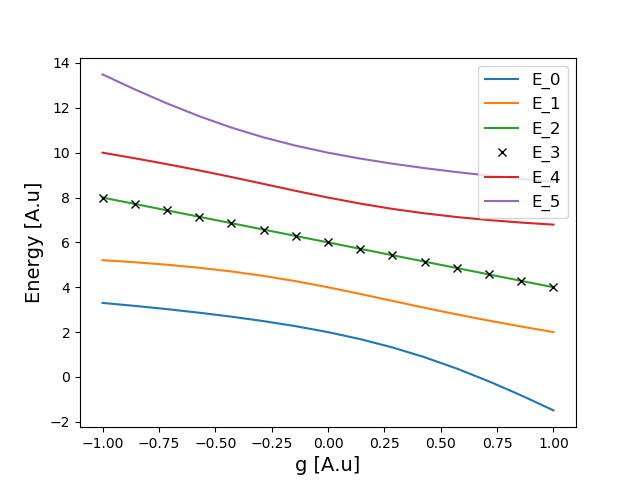
\includegraphics[width=0.8\textwidth]{eigval_vs_g.png}
\caption{The energy levels as a function of the strength $g$ for the analytic case of the pairing model. }
\label{fig: g_vs_eigval}
\end{figure}

In Figure \ref{fig: g_vs_eigval} we see the eigenvalues of the Hamiltonian matrix \eqref{eq: analytic_H_matrix} for the pairing model as a function of the strength $g \in [-1,1]$. \footnote{The diagonalization was done with \texttt{numpy}.}.

We can observe that the pairing potential increases the gap among the energy levels $E\_i$, eigenvalues of Eq.(\ref{eq: analytic_H_matrix}). The case $g=1$, corresponding to a strong attractive pairing, produces the more stable system (lowest energy levels).


\subsection{Analytic results}


are there more analytic results that we used to benchmark the code?


%------------------------------------------------


\section{Building the shell model code}

Appling the technique we learned from the pairig model in section \ref{sec:pair}, we want to extend our code to perform shell model calculation. In the specific case we build a working shell model code to describe the $O$ isotopes within the $sd$ model space. Our results will be directly compared and benchmarked to the same calculations performed with NushellX.

We construct our code step by step, keeping in mind that we are interested to describe a system with $N$ particles in the valence space.

\begin{itemize}
\item \textbf{Model space} The single-particle states are the foundamental building block of the shell model, in fact they form the so called ''basis''. In our case we read the information of the single-particle levels from file. For example \texttt{sd\_shell.sp} contains the quantum number $n$,$l$,$2j$ and $2m_j$ together with their energy levels (eigenvalue of the single-particle Hamiltonian). Looking at the energies we can notice a degeneration respect to the $m_j$ quantum number.

\item \textbf{Slater determinats} The $N$-particle wave function, solution of the Hamiltonian $H$ is a linear combination of the Slater determinants constructed inside the model space. A Slater determinant $\ket{\Phi_i}$ is a product of $N$ single-particle states different one each other (we are working with fermions and we need to satisfy Pauli principle). In \texttt{create\_table\_files.py} we calculate all possible Slater determinats and store them in \texttt{sd\_SlaterD.sd}. We work in $m$-scheme and we do not impose any condition on the total $M= \sum m_j$.
The total number of Slater determinants which can be built with $N$ particles distributed among $i$ single-particle states is
\begin{equation}
\left (\begin{array}{c} i \\ N\end{array} \right) =\frac{i!}{(i-N)!N!}. 
\end{equation}

\begin{lstlisting}[language=Python,caption=\texttt{create\_SD\_perm} uses the Python function \texttt{itertools.combinations(,)} to create all the possible Slater determinants. In the case of pairing model the Slater determinants are restricted to the ones with $\protect{M=0}$ and coupled pairs of single-particle states.]
import numpy as np
import itertools

def create_SD_perm(N_particles, nr_sp_states, sp_matrix, SD_filename, restrictions=''): 
    ...

    nr_sp_states = int(nr_sp_states)
    sp_list = []
    for i in range(1, nr_sp_states+1):
        sp_list.append(i)
    sp_tuple = tuple(sp_list)
    #print sp_tuple
    index = 0
    SD_list = []
    act_list = []
    for x in itertools.combinations(sp_tuple, N_particles):
        m_tot = 0
        for k in range (N_particles):
            m_tot = m_tot + sp_matrix[x[k]-1,4]
        #PAIRING CASE
        # only N_particles even is considered
        if restrictions == 'pair':
            if N_particles%2 == 0:
                pair_bool = 0
                # check that the single-particle states are in pairs
                for j in range (0,N_particles,2):
                    if np.array_equal(sp_matrix[x[j]-1,1:3], sp_matrix[x[j+1]-1,1:3]):
                        pair_bool = pair_bool 
                    else:
                        pair_bool = pair_bool +1
                # check that M=0 and pairs are coupled
                if m_tot == 0 and pair_bool == 0:
                    index +=1
                    SD_list.append(index)
                    SD_list.extend(list(x))
        #GENERAL CASE
        else:
            index +=1
            SD_list.append(index)
            SD_list.extend(list(x))
    
    nr_SD = index
    SD_array = np.array(SD_list)
    SD_states = SD_array.reshape(nr_SD,N_particles+1)
    ...

\end{lstlisting}


%------------------------------------------------

\item \textbf{Hamiltonian matrix} We use the Slater determinants as basis to set up the Hamiltonian matrix $H_{ij}=\bra{\Phi_i} \hat H \ket{\Phi_j}$. It is constructed in \texttt{ham.py} as sum of one-body Hamiltonian

\begin{equation}
\hat H_0 =  \sum_{p,q} \langle p \vert \hat h_0 \vert q \rangle \hat a_{p}^\dagger \hat a_{q},
\end{equation}

and two-body interaction

\begin{equation}
\hat V = \frac{1}{4} \sum_{p,q,r,s} \langle p q\vert \hat v \vert rs \rangle_{AS} \;\hat a_{p}^\dagger \hat a_{q}^\dagger \hat a_{s} \hat a_{r}.
\end{equation}
$\langle p q\vert \hat v \vert rs \rangle_{AS}$ are the two-body antisymmetrized matrix elements for the $\hat v$ interaction. We read them from the file \texttt{sd\_mscheme.int} for the interaction $usdb$ optimized in the $sd$-model space.
\item \textbf{Diagonalization} The Hamiltonian matrix is finally diagonalized using \texttt{numpy}. The eigenvalues obtained represent the energy of the $N$-particles state and the eigenvectors are the coefficient of the Slater determinants that form the many-body wave function. In our case we obtain degenerate energy levels because our Hamiltonian is not dependent from the total azimutal angular momentum $M$ then all the $M$-multiplets with same $J$ have the same energy [write it better with the comparison with NushellX that is in $J$-scheme.]
\end{itemize}




\subsection{The structure of the code}

The code is organized into blocks of code stored in separate files that performs different tasks. The files needed to run the shell model code is:
\begin{itemize}
\item \texttt{main.py}
\item \texttt{create\_table\_files.py}
\item \texttt{read\_files.py}
\item \texttt{unit\_tests.py} 
\item \texttt{ham.py} 
\item \texttt{input\_func.py}
\end{itemize}

The \texttt{main.py} program runs the code and calls the functions in the other files. The structure of the \texttt{main.py} program is as follows:

\begin{enumerate}
\item Import files (modules)
\item Ask user to provide inputs on the command line. The only inputs needed are
\begin{itemize}
\item \texttt{N\_particles} - number of valence particles (neutrons) 
\item \texttt{case} - model space 'sd' (or 'pairing')
\item \texttt{g} - strenght of the pairing (needed only in 'pairing' case)
\end{itemize}
\item Read the single-particle basis
\item Create all the possible the Slater Determinants
\item Read and store the two-body matrix elements (tbme). In the case 'pairing', create all the non-zero pairing matrix elements according to the given strenght $g$.
\item Build the total Hamiltonian matrix from the one- and two-body terms
\item Check (unit test) if the Hamiltonian for the pairing problem is correct. If not exit the program with an error message
\item Print the eigenvalues and eigenvectors of the problem
\end{enumerate}

%NOT TRUE ANYMORE Before the basis, Slater determinants and the tbme are created the program checks, for each case if the file already exist. If the file containing for instance the basis do not exist the basis will be generated and saved to file before the code reads the file. If the file with the basis already exist the code will jump to reading the file. This way we avoid creating the (same) files every time the code is run. 

\paragraph{To run the code} one simply runs the program typing from terminal
\begin{center}\texttt{python main.py}\end{center} 
and the program will interactively ask the user for input in the terminal. The user input function is implemented in such a way that the user is not allowed to provide unphysical input values. If invalid input is given the program provides an error message and asks the user to provide the input within the allowed type or interval. When the input is given the program runs and prints the results in the terminal.

\subsection{Phase and counting the difference between the Slater determinants}

It is interesting to point out the physics behind the set-up the Hamiltonian matrix $H_{ij}=\bra{\Phi_i} \hat H \ket{\Phi_j}$.
We assume $\ket{\Phi_0}$ as an ansatz for the ground state and we consider the other Slater determinants $\ket{\Phi_i}$ as particle-hole (p-h), two particles- two holes (2p-2h), ... excitations of the ground state.
In this formalism 
\begin{equation}
\ket{\Phi_0} = \hat a_{i}^\dagger \hat a_{j}^\dagger... \ket{0}
\end{equation}
has all the single-particle levels $i,j,...$ filled and we indicate that with $i,j,...\leq F$ Fermi energy.
Of consequence, we define a p-h Slater determinant with 
\begin{equation}
\ket{\Phi_i^a} = \hat a_{a}^\dagger \hat a_{i} \ket{\Phi_0}
\end{equation}
where the particle index is $a > F$ and the hole index is $i \leq F$, and a 2p-2h one with 
\begin{equation}
\ket{\Phi_{ij}^{ab}} = \hat a_{a}^\dagger \hat a_{b}^\dagger \hat a_{j} \hat a_{i} \ket{\Phi_0}
\end{equation}
where $a,b > F$ while $i,j \leq F$.

Using Wick's contractions we can calculate the expectation values of the Hamiltonian operators among the states just built:
\begin{equation}
\bra{\Phi_0} \hat H \ket{\Phi_0} = \sum_{i \leq F} \langle i \vert \hat h_0 \vert i \rangle + \frac{1}{2} \sum_{i,j \leq F} \langle i j\vert \hat v \vert ij \rangle_{AS} 
\end{equation}

\begin{equation}
\bra{\Phi_0} \hat H \ket{\Phi_i^a} =  \cancel{\langle i \vert \hat h_0 \vert a \rangle} +  \sum_{j \leq F} \langle i j\vert \hat v \vert aj \rangle_{AS} \; 
\end{equation}
where ${\langle i \vert \hat h_0 \vert a \rangle}=0$ because the single-particles states are orthogonal;
\begin{equation}
\bra{\Phi_0} \hat H \ket{\Phi_{ij}^{ab}} =  \langle i j\vert \hat v \vert ab \rangle_{AS}
\end{equation}

\begin{equation}
\bra{\Phi_0} \hat H \ket{\Phi_{ijk}^{abc}} = 0
\end{equation}
where $\ket{\Phi_0}$ and $\ket{\Phi_{ijk}^{abc}}$ (3p-3h state) differ for more than 2-particles, the maximum number that can be contracted with a two-body Hamiltonian.

Similar expressions for the Hamiltonian matrix elements can be obtained starting from $\ket{\Phi_k}$ with $k$ generic and considering the other Slater determinants that can interact with it through $\hat H$. We use this information to construct $H_{ij}$ in a more efficient way, calculating only the non-zero matrix elements.

\begin{lstlisting}[language=Python,caption=\texttt{beta\_alpha\_compare} is a function in module \texttt{compare.py} that make a comparison between $\protect{\bra{\Phi_\beta}}$ and $\protect{\ket{\Phi_\alpha}}$ to determine their difference in terms of single-particle states.]


def beta_alpha_compare(beta_list, alpha_list):
    
    phase = 0
    diff_list = []
    beta_list_red = list(beta_list)
    alpha_list_red = list(alpha_list)
    #if len(beta_list) == len(alpha_list):
    for i in range(0, len(beta_list)):
        j=0
        j_found = False
        while j < len(alpha_list) and j_found == False:
            #print beta_list[i],i, alpha_list[j],j, diff_list
            if beta_list[i] == alpha_list[j]:
                j_found = True
                alpha_list_red.remove(alpha_list[j])
                beta_list_red.remove(beta_list[i])
                #phase = phase+j+len(beta_list)-i-1
            else:
                j = j+1
    diff_list.extend(beta_list_red)
    diff_list.extend(alpha_list_red)


    for i in range(0,len(diff_list)/2):
    	phase = phase + (list(beta_list).index(diff_list[i]))
 
    for i in range(len(diff_list)/2,len(diff_list)):
        phase = phase + (list(alpha_list).index(diff_list[i]))
        
    phase = (-1)**phase

    #print diff_list, phase
    
    return diff_list, phase

\end{lstlisting}

\subsection{Unit tests and benchmarks}

(have not done this?)

One obvious case is that of removing the two-body interaction. Then we have only the single-particle energies. For the case of degenerate single-particle orbits, that is one value of total single-particle angular momentum only $j$, with degeneracy $\Omega = 2j + 1$, one can show that the ground state energy $E_0$ is with $n$ particles

\begin{equation}
E_0 = -\frac{g}{4}n (\Omega - n + 2)
\end{equation}

Enlarge now your system to six and eight fermions and to $p = 6$ and $p = 8$ single-particle states, respectively. Run your program for a degenerate single-particle state with degeneracy $\Omega$ and test against the exact result for the ground state. Introduce thereafter a finite single-particle spacing and study the results as you vary $g$, as done in b) and c). Comment your results.

(describe the unit test that we have implemented and how)



\subsection{Challenges and proposed solutions / Future work(?)}

 something about the accuracy of our code somewhere here?
 
 
 
%------------------------------------------------


Example of python code

\begin{lstlisting}[language=Python]
import numpy as np
import sys
import matplotlib.pyplot as plt


g_list = np.linspace(-1,1,15)
N = 6
E = np.zeros(len(g_list))

plt.figure(1)
for j in range(6):
    for i in range(len(g_list)):

        g = g_list[i]

        analytical_hamiltonian = -g*np.ones([N,N])
        np.fill_diagonal(analytical_hamiltonian, 2.-2.*g)
        np.fill_diagonal(np.rot90(analytical_hamiltonian), 0)

        for n in range(N):
            analytical_hamiltonian[n,n] += 2*n

        for m in range(5,2,-1):
            analytical_hamiltonian[m,m] = analytical_hamiltonian[m-1,m-1]

        eigval, eigvec = np.linalg.eigh(analytical_hamiltonian)

        E[i] = eigval[j]

    if j==3:
        plt.plot(g_list, E, 'kx')
    else:
        plt.plot(g_list, E)


plt.xlabel('g[A.u]', fontsize=14)
plt.ylabel('Energy[A.u]', fontsize=14)
plt.legend(['E_0', 'E_1', 'E_2', 'E_3', 'E_4', 'E_5'], fontsize=12)

plt.savefig('figures/eigval_vs_g.png')
#plt.show()
\end{lstlisting}


%------------------------------------------------


\section{NuShellX (and NuShellX@MSU)}

NushellX is a code developed by W. D. M. Rae [ref] that provides an powerful tool for nuclear structure calculations. With this code one can obtain exact energies, eigenvectors and spectrosopic overlaps for low-lying states in shell-model Hamiltonian matrix calculations with very large basis dimensions (write this sentence better ?). A set of wrapper codes called NuShellX@MSU is written by Alex Brown. These wrapper codes generates input for the NuShellX code and converts the output into tables and figures for energy levels, gamma decay and beta decay.

NuShellX uses the m-scheme and jj-coupling. It is written in pn-formalism; it uses a J-coupled proton-neutron the basis, the states for protons and neutrons are created separately. The code can consider J-scheme matrix dimensions of up to the order of a 100 million. To take take advantage of many cores in modern computers OpenMP for the Lanczos iterations is used. This way the code can handle quite large model spaces in a reasonable time on a laptop. 




BUT it is very easy to produce unrealistic or inappropriate calculations



The goal of our project was to create a mini-version of the NuxhellX code and (after pairing model) use the NushellX code to test our own code.




how to use the code


our results



Calculations in an infinite space are not possible – some truncation is required
-Generally, the best and most complete results are found with the largest model spaces... But the computation time increases exponentially with model space size...... And an the interaction used must be appropriate for the model space ...
... And empirical interactions are (usually) better determined for smaller model spaces (fewer TBME)
Calculations in the full model space may be too computationally intensive OR inappropriate for the interaction-->Truncatethemodelspacetomakecalculations feasible

Only subshell truncations are possible in NuShellX – limit numbers of protons (neutrons) in a given orbital. Cannot restrict the total number of nucleons in a given orbital (proton and neutrons are treated separately)







\begin{figure}[ht]
\centering
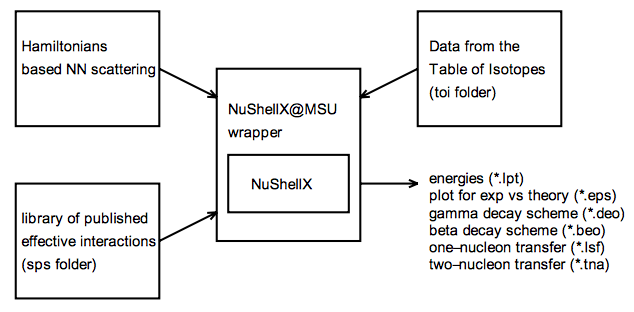
\includegraphics[width=0.8\textwidth]{nushellX_structure_from_ref.png}
\caption{Schematic layout of the NuShellX@MSU codes from ref [] }
\label{fig: nushellx_struct}
\end{figure}


reference: https://people.nscl.msu.edu/~brown/brown-all-papers/525-2014-nds120.115-nushellx.pdf
(and references within)












\section{Results}

%\begin{table}
%\caption{Example table}
%\centering
%\begin{tabular}{llr}
%\toprule
%\multicolumn{2}{c}{Name} \\
%\cmidrule(r){1-2}
%First name & Last Name & Grade \\
%\midrule
%John & Doe & $7.5$ \\
%Richard & Miles & $2$ \\
%\bottomrule
%\end{tabular}
%\end{table}




%------------------------------------------------

\section{Discussion}


%------------------------------------------------


\section{Conclusions}



%------------------------------------------------



\section*{Structure of report (crude first idea):}

\begin{enumerate}
\item Title
\item Abstract
\item Introduction
\begin{itemize}
\item Why useful
\item Where useful (nuc. chart)
\item (Look at the TALENT proposal)
\item comparing different tools
\end{itemize}
\item The Pairing problem
\begin{itemize}
\item theory
\item analytic / exact results
\end{itemize}
\item Building a shell-model code
\begin{itemize}
\item Describe the different parts/blocks of the code (basis, SD, states, int, hamiltonian...)
\item Unit tests / benchmarks (analytic/exact results)
\item Psedo code?
\item Accuracy of our code
\item Where our code fails, why and proposing solutions
\end{itemize}
\item NuShellX
\begin{itemize}
\item describe why useful / 'powerful tool' and what may be calculated
\item compare with our own code
\item Possible 'future calculations'
\end{itemize}
\item Conclusions / Summary
\end{enumerate}

%------------------------------------------------
%------------------------------------------------




%----------------------------------------------------------------------------------------
%	REFERENCE LIST
%----------------------------------------------------------------------------------------

\begin{thebibliography}{99} % Bibliography - this is intentionally simple in this template
%
%\bibitem[Figueredo and Wolf, 2009]{Figueredo:2009dg}
%Figueredo, A.~J. and Wolf, P. S.~A. (2009).
%\newblock Assortative pairing and life history strategy - a cross-cultural
%  study.
%\newblock {\em Human Nature}, 20:317--330.

\bibitem[Github of the TALENT School][ MHJ and Alex Brown
\newblock {\em link goes here},
 
\end{thebibliography}

%----------------------------------------------------------------------------------------

\end{document}
